\chapter{Implementation of domain modeling assistant}

Let us now use the delineated framework to implement a concrete modeling assistant. We define the generators with prompt templates based on the meta
template. This includes defining (1) main control instructions, modeling procedure specifications and output specifications, (2) zero or more examples for N-shot prompting, and (3) a technique for context specification.


\section{Generators configuration}

All our prompt templates can be found in our GitHub repository\footnote{\url{https://github.com/Dominik7131/Conceptual-Modeling-LLM-Assistant/tree/master/prompts}}.


\subsection{Output order}
\label{sec:output_order}

When the task of modeling domain elements solely based on a given domain description is done by the modeling experts, they typically proceed in the following two steps: (1) they find the context for the given element and (2) from the found context they extract the specific information such as name of the element.

To mimic this approach, we instruct the LLM in the output specification part to first generate the context for the given element and then to generate the specific information of this element.


\subsection{Output specification}

To the prompt we insert each structured data in the JSON format as each LLM should be greatly familiar with this format. To improve the response time of our application we instruct the LLM to output one isolated JSON object for each outputted domain element. This way as soon as the LLM generates some proper domain element it can be displayed to the user.


\subsection{Modeling procedure}

For generating classes, attributes and associations we implemented the following approaches: baseline, CoT, N-shot, CoT + N-shot. Additionally, for generating classes we implemented the ToT approach.

The table \ref{tab:main-control-instructions} shows examples of our main control instructions. These instructions are independent of the used prompting technique.

\begin{table}[!h]
    \scriptsize
    \centering
    \setlength{\tabcolsep}{0.5em}
\begin{tabular}{@{}l>{\raggedright\arraybackslash}p{0.9\textwidth}>{\raggedright\arraybackslash}p{0.5\textwidth}@{}}
         & main control instruction \\
    \toprule
    \addlinespace
    
$gen_c$ & Solely based on the given context extract all class names for a UML diagram. \\
\addlinespace

$gen_a$ & Solely based on the given context generate all attributes for the class: ``\{source\_class\}''. \\
\addlinespace

$gen_{r1}$ & Solely based on the given context which attributes does the class: ``\{source\_class\}'' have? \\
\addlinespace

$gen_{r2}$ & Solely based on the given context which associations are explicitly between the source class ``\{source\_class\}'' and the target class ``\{target\_class\}''? \\
\addlinespace

$gen_{cn}$ & Solely based on the given class description and class original text generate a class name and output this name in this JSON object: \{``name'': ``''\}. \\
\addlinespace

$gen_{ad}$ & Solely based on the given context provide description for the attribute: ``\{attribute\_name\}'' of the class: ``\{source\_class\}'' and output it in this JSON object: \{``description'': ``''\}. \\
\addlinespace

	\bottomrule
	\addlinespace
	\end{tabular}
	\caption{Examples of main control instructions}
	\label{tab:main-control-instructions}
\end{table}


\subsubsection{Chain of thoughts}

We experiment with the CoT prompting technique for generating classes, attributes and associations. First, we need to come up with a reasoning steps that the LLM can generate before it outputs each individual domain element. Some possible reasoning steps can be suggested by the LLM by adding the ``\textit{Let's think step by step}'' phrase into the prompts for generating classes, attributes and associations as discussed in the section \ref{sec:chain_of_thoughts}. Figure \ref{fig:cot-think-step-by-step} shows one of the possible reasoning steps when using ChatGPT-4o with the simple domain description from the section \ref{sec:simple_domain_description_example} for generating attributes.

\begin{figure}[!h]
    \centering
    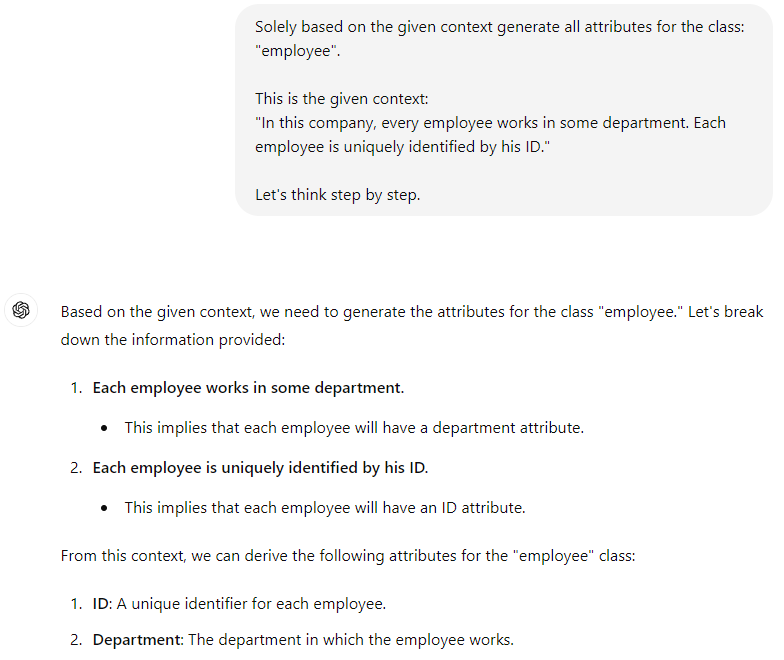
\includegraphics[scale=0.6]{img/cot-think-step-by-step.png}
    \caption{\centering Example of automatically generated reasoning steps by ChatGPT-4o for finding attributes in a simple domain description}
    \label{fig:cot-think-step-by-step}
\end{figure}

As we can see, ChatGPT-4o for each attribute first rephrased some parts of the domain description and then based on these parts it identified the possible attributes. Note that this approach is consistent with the output order that we specified in the section \ref{sec:output_order}.
Inspired by this result, we implemented a simple CoT strategy that instructs the LLM to for each domain element first generate it's original text, then generate all other fields such as the name and at the end generate all these previous items in a single JSON object. The table \ref{tab:cot-prompt-templates} shows the modeling procedures and the output specifications for $gen_c$, $gen_a$ and $gen_{r1}$.

% Other more sophisticated CoT strategies can be used. For example, when the LLM generates attributes to instruct the LLM to add for each generated domain element a reason why it thinks it is an attribute.

\begin{table}[!h]
    \scriptsize
    \centering
    \setlength{\tabcolsep}{0.5em}
\begin{tabular}{@{}l>{\raggedright\arraybackslash}p{0.4\textwidth}>{\raggedright\arraybackslash}p{0.5\textwidth}@{}}
         & modeling procedure & output specification \\
    \toprule
    \addlinespace
         $gen_c$ & For each class copy the part of the given context containing this class and output its name and then output this class in JSON object. & The output should look like this: \newline
context: copy the part of the given context containing this class \newline
name: class name \newline
JSON object: \{``originalText'': ``copy the part of the given context containing this attribute'', ``name'': ``class name''\}. \\
\addlinespace

         $gen_a$ & For each attribute copy the part of the given context containing this attribute and output its name and then output this attribute in JSON object. & The output should look like this: \newline
context: copy the part of the given context containing this attribute \newline
name: attribute name \newline
JSON object: \{``originalText'': ``copy the part of the given context containing this attribute'', ``name'': ``attribute name''\}. \\
\addlinespace

         $gen_{r1}$ & For each association output its name and source class and target class and copy the part of the given context containing this association in JSON object. &
The output should look like this: \newline
context: copy the part of the given context containing this association \newline
name: association name \newline
source class: source class name \newline
target class: target class name \newline
\{``originalText'': ``copy the part of the given context containing this association'', ``name'': ``association name'', ``source'': ``source class name'', ``target'': ``target class name''\} \\
	\addlinespace
	\bottomrule
	\addlinespace
	\end{tabular}
	\caption{Example of CoT modeling procedures and output specifications}
	\label{tab:cot-prompt-templates}
\end{table}


\subsubsection{N-shot prompting}

We use examples based on the domain description and its domain model that is shown in the figure \ref{fig:prompting-domain}.

\begin{figure}[!h]
    \centering
    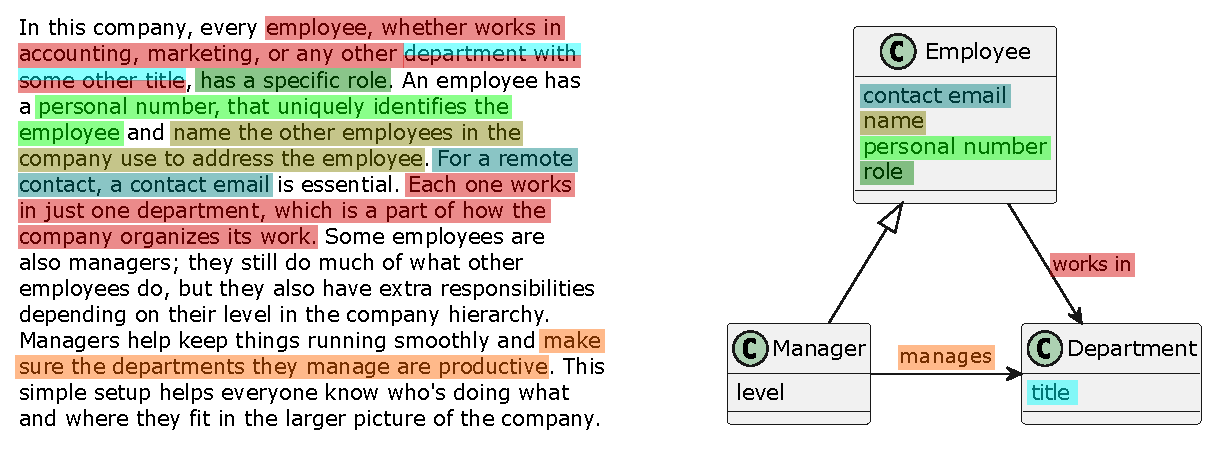
\includegraphics[scale=0.6]{img/prompting-domain.pdf}
    \caption{\centering The simple company employees domain description and its corresponding domain model used for N-shot prompting in our generator templates}
    \label{fig:prompting-domain}
\end{figure}


For $gen_c$, we use the three classes as examples. For $gen_a$, we use the colored attributes, each with the colored part of the text as examples of the corresponding original texts. For $gen_{r1}$ and ${gen_{r2}}$, we proceed similarly, but for ${gen_{r1}}$ we provide each sample association twice – for the source class and for the target class.

The concrete examples can be used to further specify the output format. For example, when the LLM is not provided with a specific name format for the corresponding domain elements, the outputted names can sometimes be in a snake case convention and some other time in a camel case convention. But when the provided examples contain a consistent naming format, the LLM usually outputs the provided format consistently. Similarly, N-shot prompting lets us specify the naming style. For example, when no naming style is provided for attributes, they can contain some unwanted words such as starting with the word ``has''.


\subsubsection{CoT + N-shot prompting}

Our combination of the CoT and the N-shot prompting technique contains the same modeling procedure as shown in the table for only CoT approach. However, the output specification part contains only the the expected JSON object and the intermediate steps are demonstrated in the part where the $N$ examples are provided.


\subsubsection{Tree of thoughts}

Even though our defined domain modeling steps are not the typical tasks that the ToT is usually used for, we tried using this technique for generating classes in the single prompt fashion as discussed in the section \ref{sec:tree_of_thoughts}.

We did not experiment with any iterative prompting technique as this would significantly increase the response time of our application as discussed in the section \ref{sec:iterative_prompting}.

% Possible iterative technique for generating classes: we could generate multiple lists of class suggestions with multiple prompts. Then we could apply some operation to these lists such as intersection or unification. Or for example, we could remove only those classes that appeared in only one list.


\subsection{Retrieval-augmented generation}

We consider the domain description $T$ as the external knowledge base and our goal is to insert only the relevant parts of the $T$ in the context specification part of the prompt. We use this technique for the generators of: attributes, associations, descriptions, data types and cardinalities as in these cases only the information about the source class $C$ is needed for generating correct output. For example, consider the following domain description: \\

\noindent{}``\textit{In this company, every employee works in some department. Each employee is uniquely identified by his ID.}''\\

\noindent{}When we want to extract attributes or associations of the class \textit{department} we are only interested in the first sentence since this is the only sentence that contains information about this class. Therefore in this case we can provide only the first sentence of the domain description into the context specification part of the prompt.

Main goal of the mentioned approach is to reduce the hallucination of the LLM such as reducing irrelevant domain elements suggestions by forcing the LLM to focus on the important parts of the domain description. Furthermore, this approach usually reduces the prompt length which can help when working with a domain description that does not fit in the context window size of the LLM.

Now we describe the most significant challenges we encountered when implementing the mentioned RAG approach and the corresponding solutions we implemented to address them.


\subsubsection{Domain description simplification}

We considered using a LLM to simplify the domain description so the LLM assistant would work only with this simplified version. However, there are a few disadvantages to this approach.

First, the LLM sometimes changes some names of the original domain elements. For example, when we instructed the ChatGPT-4o with a domain description about aircraft manufacturing and with the following prompt: \\

\noindent{}``\textit{Simplify each sentence structure in the following text. Make sure to not change any nouns and verbs as we want to keep names of all domain elements unchanged. This is the following text: \ldots}'' \\

\noindent{}The sentence: ``\textit{Customers represent the clients who purchase the finished aircraft.}'' was simplified into: ``\textit{Customers are clients who buy finished aircraft.}'' This means that the original association ``\textit{client purchases aircraft}'' was changed into ``\textit{client buys aircraft}'' which is semantically the same but it can be a problem if the user wants the suggestions to have the same name as described in the text.

The second disadvantage is that the domain description simplification removes the ability to highlight original text for each suggested domain element in the original description as the LLM works only with the simplified version of the domain description. Therefore, we do not simplify the domain description.


\subsubsection{Domain description segmentation}

In the RAG indexing phase, the domain description needs to be split into chunks so that each chunk can be evaluated if it is relevant for the given source class. Determining the chunk size is a challenging task since with too big chunks we are risking having irrelevant parts of domain description in the prompt and thus decreasing the LLM performance. On the other hand, with too small chunks we are risking that the chunks will be miss-classified as they will not contain enough information about their context for deciding if they are relevant.

In the result, we consider each sentence of the domain description as a one chunk since one sentence usually contains information about one concept or a few related concepts. The advantage of this approach is that after the chunks evaluation is done it is easy to concatenate the relevant chunks together simply by putting them next to each other in the original order from the domain description. On the other hand, the disadvantage is that for example, if some sentence refers to an another sentence with a pronoun then without any additional domain description pre-processing this context is lost during the chunks evaluation.


\subsubsection{Lack of context}

As mentioned, chunks in the form of isolated sentences can be miss-classified if not enough context is provided. This mostly happens when a sentence contains pronouns that refer to some other sentence. For example, consider the class named \textit{book} and the following domain description: \\

\noindent{}``\textit{The book contains a lot of pages. It is very heavy.}'' \\

\noindent{}Now when classifying the chunk ``\textit{It is very heavy.}'' it most likely will be classified as irrelevant chunk as in isolation it does not contain any information about the class \textit{book} even thought the attribute \textit{weight} of the \textit{book} could be inferred from it.

To solve similar issues, we implemented a simple naive algorithm where each chunk has it's own metadata and if a chunk starts with a pronoun we insert in it's metadata the previous chunk. Now when chunk is being evaluated, it's metadata are also considered. This means that when classifying the second sentence from the example also the first sentence is present therefore the context is not lost. The disadvantages of this approach are that pronouns that are not at the start of a chunk are not considered. Additionally, adding a whole previous chunk to a current chunk can in some cases lead to a current chunk miss-classification if the current chunk is not referencing the whole context of the previous chunk.

A possible better solution is to use some language model that can accurately solve the co-reference resolution task where each pronoun is replaced with the corresponding words that it references. This way when the second chunk from the example is being classified, the classification algorithm works with this text: ``\textit{The Book is very heavy}'' so all relevant context is provided. \\

Another issue with a lack of context can arise when a text contains some bullet points, such as: \\

\noindent{}``\textit{The book contains:}
\begin{itemize}
\item \textit{info about it's author}
\item \textit{date of publication}'' \\
\end{itemize}

\noindent{}To solve this issue, each of the bullet points has in it's metadata a reference to the chunk before the first bullet points which in this case is ``\textit{The book contains:}''.

In cases of some other possible chunks miss-classifications when the main goal of the assistant is to always suggest every possible domain elements then either the RAG can be temporarily disabled or the domain description can be manually edited to remove the problematic constructs.


\subsubsection{Texts comparison}
\label{texts_comparison}
  
We considered using LLM to directly output the relevant texts from the domain description based on the given source class. However, this process can take a long time as in the worst case scenario the LLM has to copy the whole domain description to the output.

Instead, we implemented a semantic and a syntactic approach that for a given source class and some part of a domain description compares their similarity.
 
The semantic approach uses an embedding model that converts input texts into a vector space and then compares their similarity.

The syntactic approach uses a language model the converts the given source class and each chunk into lemmas. Subsequently, if the chunk contains the lemmas of the given source class than it is classified as relevant. For example, consider the source class \textit{department} and the following domain description: \\

``\textit{In this company, every employee works in some department. Each employee is uniquely identified by his ID.}'' \\

First, each word in the source class \textit{department} is converted into a lemma which is again the word \textit{department}. Then, each word in the domain description is converted into the lemmas: \\

``\textit{In this company, every employee \textbf{work} in some department. Each employee \textbf{be} uniquely \textbf{identify} by his ID.}'' \\

The bold words emphasise the differences between the original domain description and the domain description after each word is converted into a lemma. Subsequently, in this case a chunk is relevant if it contains the word \textit{department}. Which in this case is only the first sentence. We do not enforce the chunk to contain the lemmas in the same order as the given source class. For example, consider the source class \textit{registration application} and the following chunk: \\

\noindent{}``\textit{Application of registration needs to be provided}'' \\

\noindent{}If the strict lemmas order would be enforced than this chunk would be classified as irrelevant for the source class \textit{registration application} which is unwanted behaviour.

Both of our RAG approaches are evaluated in the section.


\subsubsection{Top k search}
\label{sec:top_k_search}

In traditional RAG systems in the retrieval phase, a fixed number $k$ of the most relevant results are retrieved after applying the embedding model. However, in our specific application, $k$ is not a fixed number because the domain description may contain a variable number of relevant sentences. To address this variability, for our semantic RAG approach we need to set the computed score threshold. The challenge lies in the fact that the computed score is always relative to the given input. Consequently, in one scenario, sentences with a score higher than a certain threshold $x$ may be considered relevant, while in another scenario, sentences with a score higher than $x$ may be considered irrelevant. To mitigate this issue, we set the threshold based on the score of the most relevant sentence.
